\chapter{ PRE-PROCESSING AND HYPER-PARAMETER TUNING}
\label{ch:results}
This chapter focuses on image pre-processing and hyper-parameter tuning, two critical steps in optimizing machine learning models. I begin with image pre-processing, which involves reshaping and splitting the dataset to prepare it for model input. Next, I explore hyper-parameter tuning, where I adjust parameters like learning rate and dropout rate to improve model performance. These experiments were conducted using \textbf{3-Fold Cross-Validation} to ensure robust results.

\section{Image Pre-processing}
To prepare images for the model, they had to go through a pre-processing phase. This included reshaping them to (299, 299, 3) tensors (recommended for InceptionV3 model input). Changing the color map of the images to black and white, which is a common pre-processing process, was not considered because for this problem the colours of the animals have an importance to distinguish them.\\
\noindent
  Then, the data was split in 2 parts: train data and test data. The train data corresponds to 70\% of the total images, while the test data corresponds to the remaining 30\%. Test data was left aside for this section of project.\\ In order to find the best model configuration I experimented with each one of the models described while varying two hyper-parameters (learning rate and dropout rate). This way I was able to select the best values for the parameters to design the efficient model. The selection was based on the values of accuracy and loss, both for the training and validation data.\\
\clearpage
\section{Hyper-parameter Optimization}
With the goal of optimizing the model’s configuration, both of them went through an iterative process which included varying hyper-parameters, namely the learning rate  and the dropout percentage. The method applied was 3-Fold Cross-Validation.\\

Two values were experimented with for each of the two hyper-parameters. This is not ideal, but justified by the scarcity of time and low computational resources. Then, for both parameters, 3-Fold Cross-Validation was performed, and the history information was saved. This contains data about the progression of the loss function and accuracy over each epoch.\\

K-Fold Cross-Validation works by dividing the training data in K parts (or folds). Then the model will be trained on K-1 parts, and validated on the remaining part. This is done K times, ensuring that every fold will have an opportunity to have the role of validation. Then an average is made on the results. This solves the problem that the validation data used can give a poor representation of the model performance.\\
For this project, the data was divided in 3 folds mainly because of low resources and lack of available time, since the most common number of folds seem to be 5 or 10. Each 3-Fold Cross-Validation process took between 30 minutes and 1 hour
for simple neural network and about 5 hours (because of limited computation resources available) for complex neural network.\\
\begin{enumerate}
    \item \textbf{Simple Neural Net:} The images were resized to a standard format, unnecessary background elements were removed to help focus on the animal, and data augmentation techniques were applied to make the model less prone to overfitting.
    \begin{itemize}
    \item \textit{Learning Rate:} Two values for the learning rate were used: 0.01 and 0.001. Through the analysis of the charts present in Fig 4.1, it can be noted that having a higher learning rate helped reducing the train loss more quickly, even though the model didn't converge in either of the charts for 8 epochs. As the lower learning rate had less discrepancy between the train and validation loss, I decided to use it. None of the settings show good results, though.\\
   \begin{figure}[h]
    \centering
    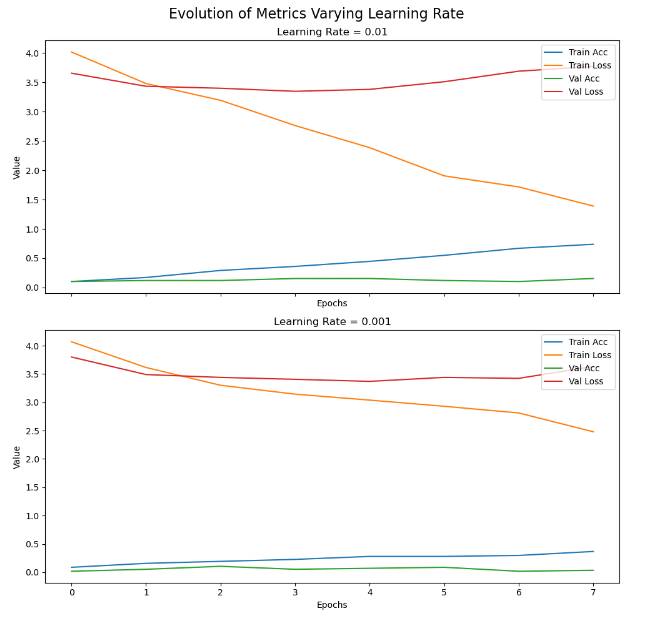
\includegraphics[width=0.7\textwidth]{figures/ssn_lr.png}
    \caption{For learning rates 0.01 and 0.001(in simple neural network)}
    \label{fig:example_images}
\end{figure}



    \item \textit{ Dropout Rate:}Another parameter observed was the dropout value. As we can see in Fig. 4.2, having a higher value lead to a lower slope of the train loss, while the other metrics stayed roughly the same. Even though neither of the two configurations showed good results, the one with the higher dropout rate was the chosen because of less difference between final values of train and validation loss.\\
   \begin{figure}[h]
    \centering
    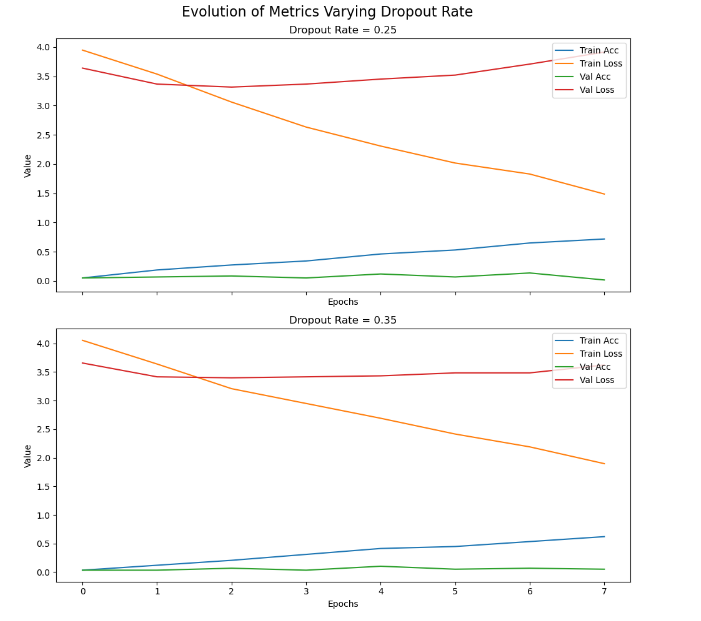
\includegraphics[width=0.7\textwidth]{figures/ssn_dr.png}
    \caption{For dropout rates 0.25 and 0.35 (in simple neural network)}
    \label{fig:example_images}
\end{figure}
\clearpage

\end{itemize}
    
    \item \textbf{Complex Neural Network:} For the more complex neural network too, I used the same parameters. I set the number of epochs to 8, and a batch size of 32. These are hyper parameters that should’ve also been through experimentation to understand the best value. But our resources didn’t allow us to perform such tasks (especially for the complex model).\\
        \begin{itemize}
    \item \textit{Learning Rate:}The values tested were 0.01 and 0.001. The graphs in Fig. 4.3 show the evolution of the accuracy and loss function, both for the train data and the validation data. As referred above, these are the average of the results from all the iterations in the 3-Fold Cross Validation.\\


From the graphs, it is clear how the lower learning rate benefits the model. The accuracy’s of both the training and validation show similar curves and the train loss is also similar. The biggest difference is in the validation loss. With the larger learning rate, this curve did not converge to a value, probably because it was “hopping” through the local minimum, due to the larger step. Thus, I concluded that the 0.001 is the best learning rate of all compared.\\
\begin{figure}[h]
    \centering
    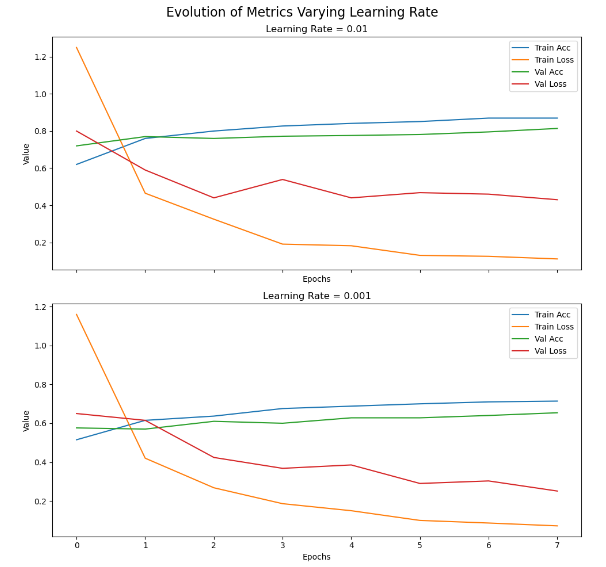
\includegraphics[width=0.7\textwidth]{figures/learning rate graph.png}
    \caption{For learning rates 0.01 and 0.001 (in complex neural network)}
    \label{fig:example_images}
\end{figure}
\clearpage

    \item \textit{ Dropout:}The values 0.25 and 0.35 were experimented with. Similar to the learning rate, the charts in Fig. 4.4 show evolution of the metrics along the 8 epochs.\\



     In this case, the differences are less noticeable. The train accuracy with 0.25 dropout is higher only by a small value in the last epoch, and also has a lower train loss by approximately 0.037. Whereas for the validation data, the accuracy is lower by a small value than with a 0.35 dropout, and has a larger validation loss by 0.025. So, there isn’t a clear “winner” here, but it will be assumed that 0.35 is better value because of the slightly better average results in the validation data.
        \begin{figure}[h]
    \centering
    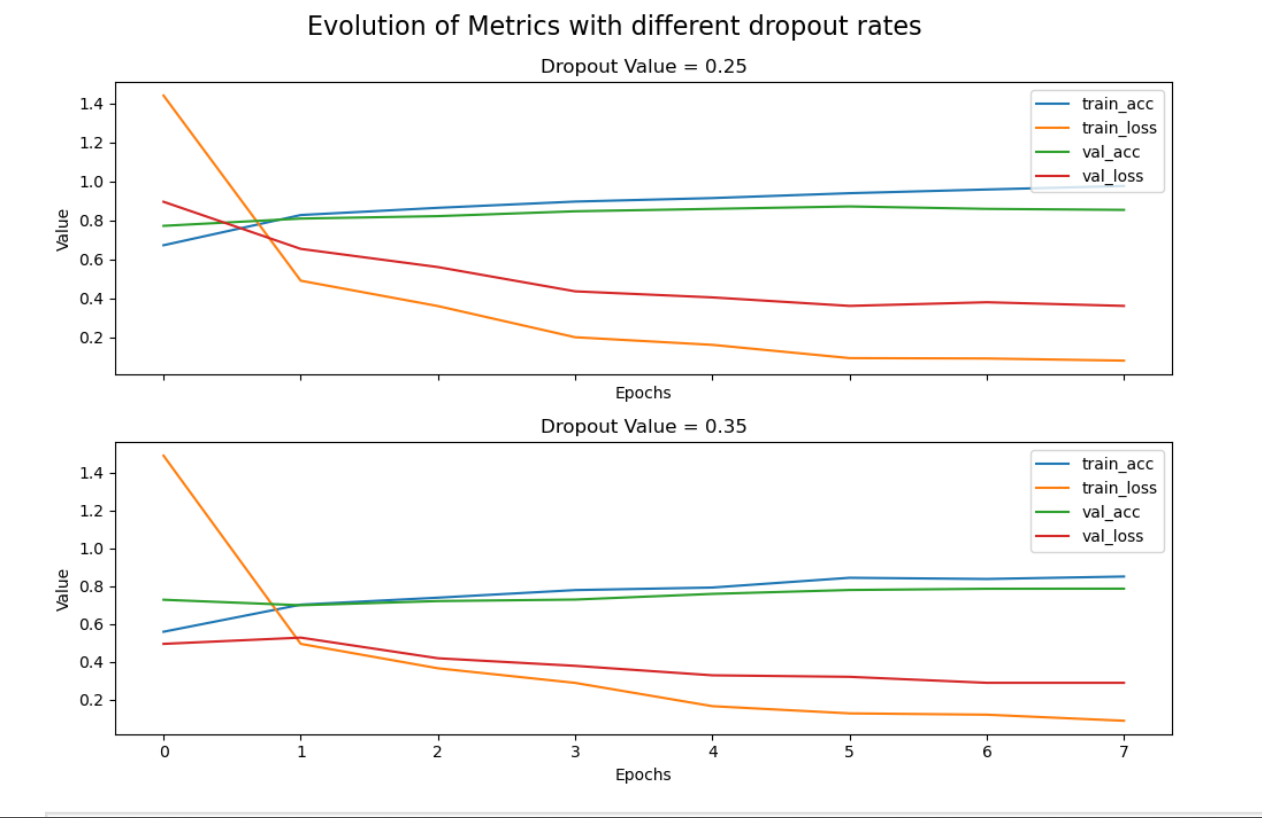
\includegraphics[width=0.7\textwidth]{figures/dropout graph.png}
    \caption{For dropout rates 0.25 and 0.35 (in complex neural network)}
    \label{fig:example_images}
\end{figure}

     

\end{itemize}
    

\end{enumerate}

\section{Summary}
In this chapter, I covered the essential steps of image pre-processing and hyper-parameter tuning to optimize the model. Image pre-processing included reshaping images to fit the InceptionV3 model and splitting the data into training and test sets, ensuring consistent input and retaining crucial color information. Hyper-parameter tuning involved adjusting key settings, such as learning rate and dropout rate, through 3-Fold Cross-Validation to improve accuracy and reduce loss. These steps helped achieve a more balanced model with better generalization.



